\documentclass[pdflatex,sn-mathphys-num]{sn-jnl}% Math and Physical Sciences Numbered

\usepackage{graphicx}%
\usepackage{multirow}%
\usepackage{amsmath,amssymb,amsfonts}%
\usepackage{amsthm}%
\usepackage{mathrsfs}%
\usepackage[title]{appendix}%
\usepackage{xcolor}%
\usepackage{textcomp}%
\usepackage{manyfoot}%
\usepackage{booktabs}%
\usepackage{multicol}
\usepackage{fancyvrb}
\usepackage{geometry}
\usepackage{titlesec}
\usepackage{xcolor}
\usepackage{parskip}
\usepackage{array}
\usepackage{multirow}
\usepackage{booktabs}
% Commented out biblatex because sn-jnl class loads natbib (incompatible)
% If you need bibliographies, use natbib commands: \citep{}, \citet{}, \bibliography{}
% \usepackage[backend=biber,style=apa]{biblatex}
% \addbibresource{references.bib}
\usepackage{hyperref}
\usepackage{xurl}             % Permite que los \url{} largos hagan salto de línea en cualquier caracter (evita overfull hbox en la sección de Referencias)
\usepackage{fontawesome5} % For the GitHub icon
\usepackage[justification=centering]{caption}
\usepackage[linesnumbered,ruled,vlined]{algorithm2e}
\setlength{\topmargin}{-0.4in}
\setlength{\textheight}{9in}
\usepackage{comment}
\usepackage{listings}%
% In your preamble:
\usepackage{enumitem} % For custom list formatting
\newlist{questions}{enumerate}{1}
\setlist[questions,1]{
  label=\textbf{Q\arabic*:}, % Label format "Q1:", "Q2:", ...
  leftmargin=2em,           % Indent spacing
  itemsep=1em               % Space between questions
}



%%%%



\raggedbottom



% Code Packages

\usepackage{listings}
\usepackage{xcolor}

\definecolor{headerbackground}{rgb}{1, 1, 1}
\definecolor{rulecolor}{rgb}{0.7, 0.7, 0.7}

% Define C keywords including standard library functions
\lstdefinestyle{algorithmstyle}{
  backgroundcolor=\color{white},
  basicstyle=\ttfamily\scriptsize,
  keywordstyle=\bfseries, % Bold for keywords
  commentstyle=\itshape, % Italic for comments
  stringstyle=,
  numberstyle=\tiny,
  numbers=left,
  numbersep=10pt,
  breaklines=true,
  frame=trbl,
  framerule=0.8pt,
  rulecolor=\color{rulecolor},
  framesep=5pt,
  xleftmargin=15pt,
  xrightmargin=5pt,
  language=C, % This is crucial
  tabsize=2,
  showstringspaces=false,
  alsoletter={\_},
  morekeywords={printf, scanf, malloc, free, sizeof, puts, gets}, % Add standard library functions
}

% ============================================ %
% Configuración adicional agregada para el      %
% reporte de CAN Bus (protocolo CAN)            %
% ============================================ %
\usepackage{siunitx}          % Unidades (Mbit/s, ns, V, etc.)
\sisetup{per-mode=symbol}
\usepackage{tabularx}         % Columnas que ajustan su ancho al \linewidth (evita tablas desbordadas)
\usepackage{ragged2e}         % \RaggedRight dentro de columnas X (mejor que justificado forzado)
\newcolumntype{Y}{>{\RaggedRight\arraybackslash}X}

% Resaltado rápido de bits dominantes/recesivos dentro del texto
\newcommand{\dominant}{\textbf{dominante (0)}}
\newcommand{\recessive}{\textbf{recesivo (1)}}

\newcommand{\codeheader}[1]{%
  \noindent%
  \fcolorbox{rulecolor}{headerbackground}{%
    \makebox[\dimexpr\linewidth-2\fboxsep-2\fboxrule][l]{%
      \textbf{Code:} \ttfamily{#1}%
    }%
  }%
  \vspace{-0.5\baselineskip}
}

\begin{document}

\title[Article Title]{Protocolo CAN (Controller Area Network): Fundamentos, Arquitectura de Trama y Aplicaciones}

\author*[1,2]{\fnm{Contreras R} \sur{Orlando}}\email{\{al348390,al464376\}@edu.uaa.mx}

\affil[3]{\orgdiv{Department of Electronic Systems}, \orgname{UAA}, \orgaddress{\street{Av. Universidad 940}, \city{Aguascalientes}, \postcode{20131}, \state{Aguascalientes}, \country{México}}}

%%==================================%%
%% Sample for unstructured abstract %%
%%==================================%%

\abstract{El presente reporte estudia el protocolo de comunicación serial \textit{Controller Area Network} (CAN), desarrollado originalmente por Bosch para reducir el cableado en sistemas automotrices. Se abordan sus fundamentos eléctricos y de capa física, la estructura de sus tramas, el mecanismo de arbitraje sin pérdida basado en \textit{CSMA/CR}, el manejo y clasificación de errores, así como su evolución hacia CAN FD. Se discuten ventajas y desventajas frente a otros buses de campo, sus aplicaciones actuales en la industria automotriz e industrial, y se presenta una guía práctica de implementación del periférico bxCAN en un microcontrolador STM32.}

\keywords{CAN Bus, ISO 11898, Bus de campo, Arbitraje, STM32, Comunicación serial, CAN FD.}

\maketitle

\section{Introducción}\label{sec1}
El protocolo \textbf{CAN (Controller Area Network)} es un estándar de comunicación serial multi-maestro diseñado para permitir que microcontroladores y dispositivos se comuniquen entre sí sin necesidad de una computadora central, dentro de un mismo sistema. A diferencia de protocolos punto a punto como SPI o UART, CAN fue concebido desde su origen como un bus multi-nodo: todos los dispositivos ``escuchan'' el mismo par de cables y deciden, mediante un mecanismo de arbitraje, quién tiene el derecho de transmitir en cada instante.

Su principal motivación histórica fue la reducción drástica del cableado en los vehículos, donde cada vez más unidades de control electrónico (ECUs) necesitaban intercambiar información (velocidad, temperatura, posición del acelerador, estado de frenos, etc.). En lugar de tender un cable dedicado entre cada par de módulos, CAN permite que todos los nodos compartan un único bus físico de dos hilos.
\begin{comment}
--------------------------------------------------------------
 IMAGEN 1: Buscar un diagrama comparativo entre "cableado      
 punto a punto tradicional en un vehículo" vs "topología de    
 bus CAN". Se espera ver, del lado izquierdo, múltiples ECUs   
 conectadas entre sí por cables individuales (maraña de        
 cables) y del lado derecho las mismas ECUs conectadas a un    
 único bus lineal de dos hilos (CAN_H / CAN_L).                
 Buscar en: "CAN bus vs point to point wiring diagram          
 automotive ECU", Bosch CAN bus wiring comparison               
--------------------------------------------------------------%
\end{comment}

\begin{figure}[!h]
    \centering
    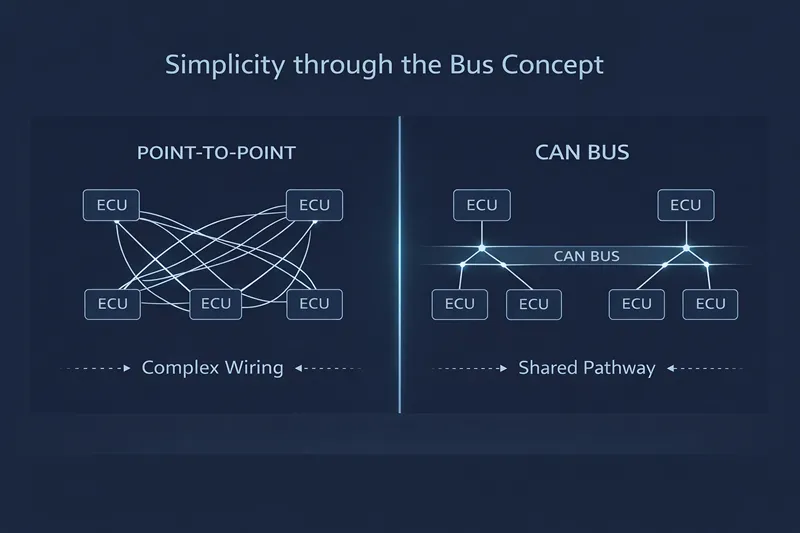
\includegraphics[width=0.8\linewidth]{src/WiringComparison.png}
    \caption{Comparación entre cableado punto a punto tradicional y topología de bus CAN}
    \label{fig:wiring_comparison}
\end{figure}

\section{Breve Historia}\label{sec:history}
El desarrollo de CAN inició en 1983 dentro de Robert Bosch GmbH, liderado por Uwe Kiencke, como respuesta a la necesidad de un bus serial robusto que redujera el cableado automotriz. El protocolo se presentó públicamente en 1986 durante el congreso SAE en Detroit, y poco después Intel y Philips (NXP) lanzaron los primeros controladores CAN comerciales.

Mercedes-Benz fue el primer fabricante en integrar CAN en un vehículo de producción, el Clase S W140, en 1991; ese mismo año Bosch publicó la especificación CAN 2.0 (con las variantes 2.0A de identificador estándar de 11 bits y 2.0B de identificador extendido de 29 bits). En 1993 la ISO ratificó el protocolo como \textbf{ISO 11898}, consolidándolo como estándar internacional. A mediados de los años 90, CAN se incorporó a los sistemas de diagnóstico OBD-II, obligatorios en Estados Unidos desde 1996.

Con el crecimiento en la cantidad de datos a transmitir por los sistemas ADAS y de infoentretenimiento, Bosch introdujo en 2012 el protocolo \textbf{CAN FD} (\textit{Flexible Data-Rate}), formalizado por ISO en 2015 dentro de ISO 11898-1:2015, permitiendo cargas útiles de hasta 64 bytes y una fase de datos a mayor velocidad.

\section{Conceptos Básicos}\label{sec:basics}

\subsection{Topología y Capa Física}
CAN utiliza un bus diferencial de dos hilos, denominados \textbf{CAN\_H} (\textit{CAN High}) y \textbf{CAN\_L} (\textit{CAN Low}). La información no se codifica como un nivel absoluto de voltaje respecto a tierra, sino como la \textit{diferencia de tensión} entre ambas líneas, lo que otorga a CAN una alta inmunidad al ruido electromagnético, característica esencial en el entorno automotriz.

Existen dos estados posibles en el bus:
\begin{itemize}
    \item \textbf{Estado recesivo (bit 1):} Ambas líneas se encuentran aproximadamente al mismo potencial (típicamente 2.5V), por lo que la diferencia de voltaje es cercana a 0V.
    \item \textbf{Estado dominante (bit 0):} CAN\_H se eleva (aprox. 3.5V) y CAN\_L desciende (aprox. 1.5V), generando una diferencia de aproximadamente 2V.
\end{itemize}

El estado dominante siempre ``gana'' sobre el recesivo cuando dos o más nodos transmiten simultáneamente, lo cual es la base física que permite el arbitraje sin colisiones (sección \ref{sec:arbitration}).

\begin{comment}
%--------------------------------------------------------------%
 IMAGEN 2: Buscar un diagrama de niveles de voltaje CAN_H y    
 CAN_L en el tiempo, mostrando el estado recesivo (ambas       
 líneas en ~2.5V) y el estado dominante (CAN_H en ~3.5V,       
 CAN_L en ~1.5V), con la diferencia de voltaje resultante.     
 Buscar en: "CAN bus CAN_H CAN_L voltage levels dominant       
 recessive diagram", ISO 11898-2 differential voltage diagram  
%--------------------------------------------------------------%
\end{comment}

\begin{figure}[!h]
    \centering
    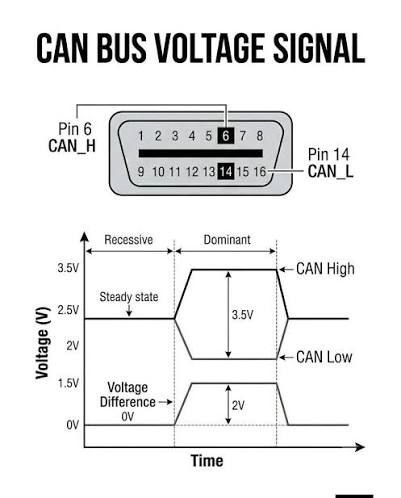
\includegraphics[width=0.5\linewidth]{src/CanVoltageLevels.png}
    \caption{Niveles de voltaje diferencial: estado dominante vs recesivo}
    \label{fig:voltage_levels}
\end{figure}

Físicamente, cada nodo se conecta al bus mediante un \textbf{transceptor CAN} (por ejemplo, el TJA1050, TJA1057, MCP2551 o SN65HVD230), que traduce los niveles lógicos TTL del controlador CAN integrado en el microcontrolador (como el periférico bxCAN o FDCAN de la familia STM32) a los niveles diferenciales del bus físico. En ambos extremos del bus se colocan resistencias de terminación de \SI{120}{\ohm} para evitar reflexiones de señal, dando una resistencia diferencial total de \SI{60}{\ohm}.

\subsection{Arbitraje y Acceso Múltiple: CSMA/CR}\label{sec:arbitration}
CAN es un bus \textbf{multi-maestro}: cualquier nodo puede iniciar una transmisión cuando detecta el bus libre. Para resolver el caso en que dos o más nodos transmiten al mismo tiempo, CAN emplea un mecanismo llamado \textbf{CSMA/CR} (\textit{Carrier Sense Multiple Access with Collision Resolution}), también descrito como arbitraje bit a bit no destructivo.

El procedimiento es el siguiente: mientras se transmite el campo de identificador, cada nodo transmisor monitorea simultáneamente el estado real del bus. Si un nodo transmite un bit recesivo pero detecta que el bus está en estado dominante (porque otro nodo transmitió un 0 en esa misma posición), dicho nodo pierde el arbitraje, deja de transmitir inmediatamente y pasa a modo receptor, reintentando su transmisión cuando el bus vuelva a estar libre. El nodo cuyo identificador contiene el valor numérico más bajo -es decir, más bits dominantes al inicio- gana el arbitraje y continúa transmitiendo sin interrupción.

Esta característica implica que \textbf{el identificador de un mensaje CAN determina directamente su prioridad}: entre menor sea el valor numérico del identificador, mayor es su prioridad en el bus. Además, este mecanismo asegura que el mensaje de mayor prioridad nunca se pierde ni se corrompe por la colisión, a diferencia de protocolos como Ethernet clásico (CSMA/CD), donde ambas tramas en colisión se descartan y deben retransmitirse.
\begin{comment}
%--------------------------------------------------------------%
 IMAGEN 3: Buscar un diagrama de temporización que muestre 3   
 nodos (Nodo A, B, C) transmitiendo sus identificadores bit a  
 bit simultáneamente, donde se observe en qué bit cada nodo    
 pierde el arbitraje al transmitir un recesivo mientras el bus 
 está dominante, hasta que un solo nodo continúa transmitiendo.
 Buscar en: "CAN bus bitwise arbitration diagram three nodes", 
 Vector CAN CSMA/CR arbitration timing diagram                 
%--------------------------------------------------------------%
\end{comment}


\begin{figure}[!h]
    \centering
    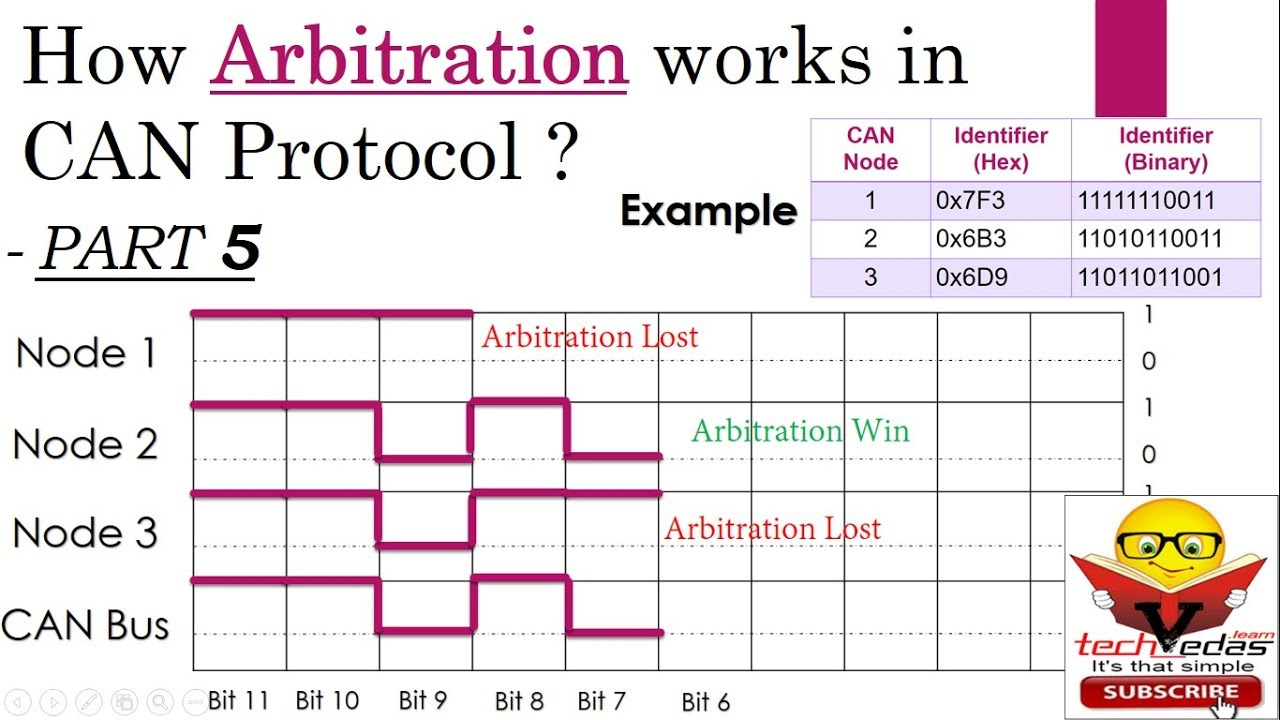
\includegraphics[width=\linewidth]{src/Arbitration.png}
    \caption{Arbitraje bit a bit (CSMA/CR) entre tres nodos compitiendo por el bus}
    \label{fig:arbitration}
\end{figure}

\section{Estructura de la Trama CAN}\label{sec:frame}
CAN define cuatro tipos de tramas: \textbf{trama de datos} (transporta información), \textbf{trama remota} (solicita datos a otro nodo), \textbf{trama de error} (señaliza una violación del protocolo) y \textbf{trama de sobrecarga} (retrasa el siguiente envío cuando un nodo requiere más tiempo de procesamiento). La trama de datos es la más relevante para el uso cotidiano del bus y se describe a detalle a continuación.

\subsection{Trama de Datos: Formato Estándar (CAN 2.0A)}
El identificador estándar utiliza 11 bits. Los campos de la trama, en orden de transmisión, son:
\begin{figure}[!h]
    \centering
    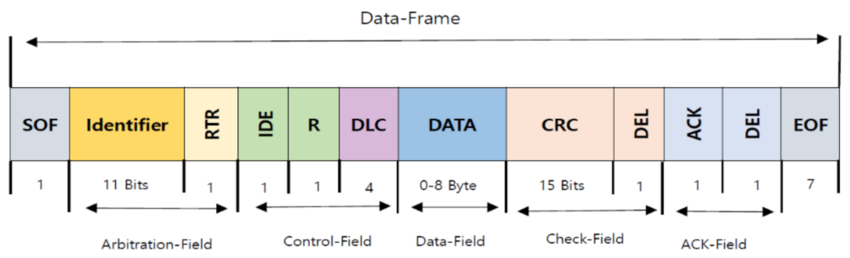
\includegraphics[width=\linewidth]{src/StandartFrame.png}
    \caption{Estructura completa de la trama de datos CAN estándar (CAN 2.0A)}
    \label{fig:standard_frame}
\end{figure}
\begin{table}[!h]
\centering
\caption{Campos de la trama de datos CAN estándar (11 bits)}
\label{tab:standard_frame}
\begin{tabularx}{\linewidth}{|>{\RaggedRight\arraybackslash}p{2.6cm}|>{\RaggedRight\arraybackslash}p{2.4cm}|Y|}
\hline
\textbf{Campo} & \textbf{Tamaño} & \textbf{Descripción} \\ \hline
SOF (Start of Frame) & 1 bit & Bit dominante que marca el inicio de la trama y sincroniza a todos los nodos. \\ \hline
Identificador & 11 bits & Define la prioridad del mensaje y, típicamente, su significado/contenido. \\ \hline
RTR & 1 bit & Dominante en trama de datos, recesivo en trama remota. \\ \hline
IDE & 1 bit & Dominante: indica formato estándar (11 bits). \\ \hline
r0 & 1 bit & Bit reservado (dominante, reservado para uso futuro). \\ \hline
DLC (Data Length Code) & 4 bits & Indica el número de bytes de datos (0 a 8). \\ \hline
Campo de datos & 0--8 bytes & Carga útil del mensaje. \\ \hline
CRC & 15 bits + 1 delimitador & Checksum para detección de errores de transmisión. \\ \hline
ACK & 1 bit + 1 delimitador & Bit de reconocimiento: el transmisor lo envía recesivo, cualquier receptor que reciba correctamente lo fuerza a dominante. \\ \hline
EOF (End of Frame) & 7 bits recesivos & Marca el final de la trama. \\ \hline
\end{tabularx}
\end{table}
\begin{comment}
    
%--------------------------------------------------------------%
 IMAGEN 4: Buscar un diagrama de la trama de datos CAN         
 estándar completa, mostrando de izquierda a derecha cada uno  
 de los campos (SOF, Identificador de 11 bits, RTR, IDE, r0,   
 DLC, Datos, CRC, delimitador CRC, ACK, delimitador ACK, EOF)   
 con su tamaño en bits marcado debajo de cada bloque.           
 Buscar en: "CAN bus standard data frame format diagram 11     
 bit identifier", ISO 11898 CAN frame structure diagram        
%--------------------------------------------------------------%
\end{comment}



\subsection{Trama de Datos: Formato Extendido (CAN 2.0B)}
El formato extendido amplía el identificador a 29 bits para admitir un mayor número de mensajes únicos, requerido por protocolos de capa superior como J1939. Se logra dividiendo el identificador en un identificador base de 11 bits y una extensión de 18 bits adicionales, separados por los bits \textbf{SRR} (\textit{Substitute Remote Request}) e \textbf{IDE} (que en este caso se transmite recesivo para indicar formato extendido).

Es importante destacar que, gracias al bit IDE, un identificador estándar siempre tiene mayor prioridad que un identificador extendido cuando ambos compiten en el mismo bit de arbitraje, ya que IDE se transmite dominante en tramas estándar y recesivo en tramas extendidas.

\subsection{Bit Stuffing}
Para garantizar suficientes transiciones de señal que permitan a los nodos mantener sincronía de reloj (recordemos que CAN es asíncrono, sin línea de reloj dedicada), el protocolo inserta un \textbf{bit de relleno (stuff bit)} de polaridad opuesta después de cada secuencia de 5 bits consecutivos del mismo valor, dentro de los campos comprendidos entre el SOF y el CRC. El receptor elimina automáticamente estos bits de relleno al reconstruir el mensaje original. Esta técnica también resulta clave para la detección de errores de relleno (\textit{stuff error}), descrita en la sección \ref{sec:errors}.

\subsection{Trama Remota, de Error y de Sobrecarga}
\begin{itemize}
    \item \textbf{Trama remota (Remote Frame):} Idéntica en estructura a la trama de datos, pero con el bit RTR recesivo y sin campo de datos. Se utiliza para solicitar a otro nodo que transmita la información asociada a un identificador específico.
    \item \textbf{Trama de error (Error Frame):} Se compone de una \textit{bandera de error} (6 bits del mismo valor, violando la regla de bit stuffing intencionalmente) seguida de un \textit{delimitador de error} (8 bits recesivos). Cualquier nodo que detecte una de las condiciones de error descritas en \ref{sec:errors} transmite esta trama para abortar la transmisión en curso.
    \item \textbf{Trama de sobrecarga (Overload Frame):} Estructuralmente similar a la trama de error, pero se genera cuando un nodo necesita más tiempo antes de procesar el siguiente mensaje, insertando un retraso adicional entre tramas.
\end{itemize}

\section{Manejo y Clasificación de Errores}\label{sec:errors}
Uno de los aspectos más robustos de CAN es su sofisticado sistema de detección de errores, que le permite alcanzar una probabilidad de error no detectado extremadamente baja. El protocolo define cinco mecanismos de detección:

\begin{table}[!h]
\centering
\caption{Tipos de error detectados por el protocolo CAN}
\label{tab:error_types}
\begin{tabular}{|l|p{7.5cm}|}
\hline
\textbf{Tipo de error} & \textbf{Descripción} \\ \hline
Bit Error & El transmisor compara cada bit enviado contra el nivel real del bus (fuera de la fase de arbitraje) y detecta una discrepancia. \\ \hline
Stuff Error & Se reciben 6 bits consecutivos del mismo valor donde debería existir un bit de relleno. \\ \hline
CRC Error & El CRC calculado por el receptor no coincide con el CRC recibido en la trama. \\ \hline
Form Error & Un campo de formato fijo (como el delimitador de CRC, ACK o el EOF) contiene un valor inválido. \\ \hline
ACK Error & El transmisor no detecta el bit de reconocimiento dominante, indicando que ningún nodo recibió la trama correctamente. \\ \hline
\end{tabular}
\end{table}

Cada nodo mantiene dos contadores internos, \textbf{TEC} (\textit{Transmit Error Counter}) y \textbf{REC} (\textit{Receive Error Counter}), que se incrementan al detectar errores y se decrementan con transmisiones/recepciones exitosas. En función del valor de estos contadores, un nodo transita entre tres estados:

\begin{itemize}
    \item \textbf{Error Active:} Estado normal de operación; el nodo participa activamente en el bus y puede emitir tramas de error activas (dominantes).
    \item \textbf{Error Passive:} Se alcanza cuando TEC o REC superan 127; el nodo continúa comunicándose pero sus tramas de error pasan a ser pasivas (recesivas), para no interferir agresivamente con el bus.
    \item \textbf{Bus Off:} Se alcanza cuando TEC supera 255; el nodo se desconecta completamente del bus para evitar comprometer la comunicación del resto de la red, requiriendo una secuencia de recuperación definida por el estándar.
\end{itemize}
\begin{comment}
    
%--------------------------------------------------------------%
 IMAGEN 5: Buscar un diagrama de máquina de estados que        
 muestre las transiciones entre "Error Active", "Error         
 Passive" y "Bus Off" en función de los contadores TEC/REC,    
 con las flechas de transición etiquetadas con las condiciones 
 (p. ej. TEC/REC > 127, TEC > 255, recuperación tras 128        
 secuencias de 11 bits recesivos).                              
 Buscar en: "CAN bus error state machine diagram error active   
 error passive bus off", ISO 11898-1 fault confinement diagram  
%--------------------------------------------------------------%
\end{comment}

\begin{figure}[!h]
    \centering
    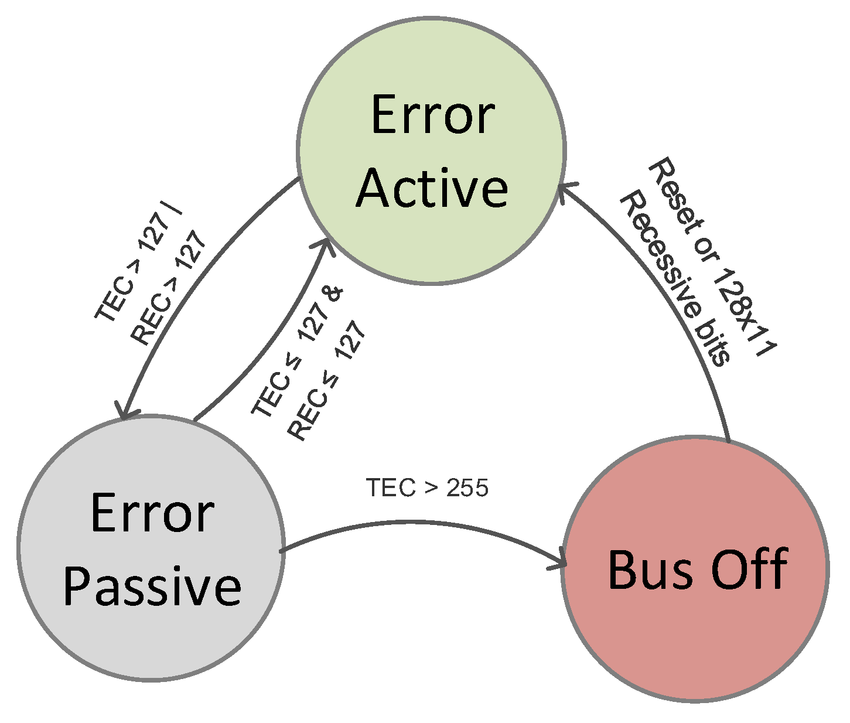
\includegraphics[width=.4\linewidth]{src/ErrorStateMachine.png}
    \caption{Máquina de estados de confinamiento de fallas (fault confinement)}
    \label{fig:error_states}
\end{figure}

\section{Capa Física: Variantes de CAN}\label{sec:physical}
El estándar ISO 11898 se subdivide en varias partes, de las cuales destacan dos variantes de capa física de uso común:

\begin{itemize}
    \item \textbf{High-Speed CAN (ISO 11898-2):} Permite velocidades de hasta \SI{1}{\mega\bit\per\second}, utilizado en aplicaciones sensibles al tiempo como el control del motor y frenos ABS. No es tolerante a fallas por sí mismo (una falla en una de las dos líneas puede detener la comunicación).
    \item \textbf{Low-Speed Fault-Tolerant CAN (ISO 11898-3):} Alcanza hasta \SI{125}{\kilo\bit\per\second}, pero puede seguir operando en modo degradado utilizando una sola línea si la otra falla (por ejemplo, corto a tierra o a alimentación), a costa de menor velocidad. Se usa en sistemas de confort (elevadores de cristal, luces, asientos).
\end{itemize}

\section{CAN FD (Flexible Data-Rate)}\label{sec:canfd}
CAN FD, introducido por Bosch en 2012 y formalizado en ISO 11898-1:2015, extiende el protocolo CAN clásico manteniendo compatibilidad con el hardware existente en la fase de arbitraje. Sus mejoras principales son:

\begin{itemize}
    \item \textbf{Carga útil ampliada:} El campo de datos crece de un máximo de 8 bytes a hasta 64 bytes por trama.
    \item \textbf{Velocidad de datos variable:} Una vez resuelto el arbitraje (que se mantiene a la velocidad nominal por compatibilidad), la fase de transmisión de datos puede conmutar a una velocidad más alta, ya que en ese punto solo un nodo transmite y no es necesario mantener los tiempos de propagación conservadores del arbitraje.
    \item \textbf{Mayor robustez del CRC:} Se emplea un polinomio CRC más robusto (17 o 21 bits, dependiendo de la longitud de datos) dado el mayor tamaño de carga útil.
\end{itemize}

Esta evolución responde al crecimiento en la cantidad de datos que deben intercambiar los sistemas ADAS, cámaras y unidades de infoentretenimiento modernas, sin necesidad de migrar a un bus completamente distinto.

\section{Ventajas y Desventajas}\label{sec:proscons}

\begin{table}[!h]
\centering
\caption{Ventajas y desventajas del protocolo CAN}
\label{tab:proscons}
\begin{tabular}{|p{6.8cm}|p{6.8cm}|}
\hline
\textbf{Ventajas} & \textbf{Desventajas} \\ \hline
Reduce drásticamente el cableado al usar un bus compartido de dos hilos. & Ancho de banda limitado (1 Mbit/s en CAN clásico), insuficiente para video o grandes flujos de datos. \\ \hline
Alta inmunidad al ruido gracias a la señalización diferencial. & Carga útil máxima de solo 8 bytes en CAN clásico, generando overhead relativo alto en mensajes pequeños. \\ \hline
Arbitraje sin pérdida: el mensaje de mayor prioridad nunca se corrompe por colisiones. & Sin direccionamiento de origen/destino nativo; cualquier nodo puede inyectar tramas con cualquier identificador (relevante en ciberseguridad). \\ \hline
Detección de errores robusta (CRC, bit stuffing, múltiples verificaciones), muy baja tasa de error no detectado. & Requiere transceptor dedicado y terminación adecuada; una falla de terminación degrada toda la red. \\ \hline
Estándar maduro, ampliamente soportado por microcontroladores (bxCAN, FDCAN) y bajo costo de implementación. & Escalabilidad limitada en número de nodos y longitud de bus a altas velocidades (dependencia del tiempo de propagación). \\ \hline
Determinismo en la prioridad de mensajes críticos gracias al identificador. & Sin cifrado ni autenticación en el protocolo base; toda la seguridad se delega a capas superiores. \\ \hline
\end{tabular}
\end{table}

\section{Aplicaciones y Uso Actual}\label{sec:applications}
Aunque CAN nació en el sector automotriz, su robustez y bajo costo lo han llevado a diversificarse en múltiples industrias:

\begin{itemize}
    \item \textbf{Automotriz:} Comunicación entre ECUs de motor, transmisión, frenos ABS/ESP, airbags, y diagnóstico OBD-II. Es la base de los buses de confort y de tren motriz en la gran mayoría de vehículos actuales.
    \item \textbf{Vehículos comerciales y agrícolas:} El estándar \textbf{SAE J1939}, construido sobre CAN de identificador extendido, define la comunicación entre ECUs en camiones, tractores y maquinaria pesada.
    \item \textbf{Automatización industrial:} El protocolo de capa de aplicación \textbf{CANopen} se utiliza extensamente en controladores de motores, sensores y PLCs industriales.
    \item \textbf{Electrónica marina:} El estándar \textbf{NMEA 2000}, basado en CAN, interconecta instrumentos de navegación, GPS y sensores en embarcaciones.
    \item \textbf{Aeroespacial y ferroviario:} Variantes de CAN se emplean en sistemas de control no críticos para la seguridad de vuelo, así como en trenes para puertas, climatización e iluminación.
    \item \textbf{Robótica y proyectos embebidos:} Muy común en drones (por ejemplo, buses CAN en controladoras de vuelo modernas para ESCs) y en robots móviles multi-nodo, dado el bajo costo de los transceptores y el soporte nativo en microcontroladores STM32, entre otros.
\end{itemize}
\begin{comment}
    
%--------------------------------------------------------------%
 IMAGEN 6: Buscar una fotografía o diagrama de red CAN dentro   
 de un vehículo mostrando múltiples buses (powertrain CAN,      
 comfort CAN, infotainment CAN) conectados a un gateway central 
 con las diferentes ECUs distribuidas en cada bus.              
 Buscar en: "automotive CAN bus network topology gateway ECU    
 diagram powertrain comfort", vehicle multiple CAN bus diagram  
%--------------------------------------------------------------%
\end{comment}

\begin{figure}[!h]
    \centering    
    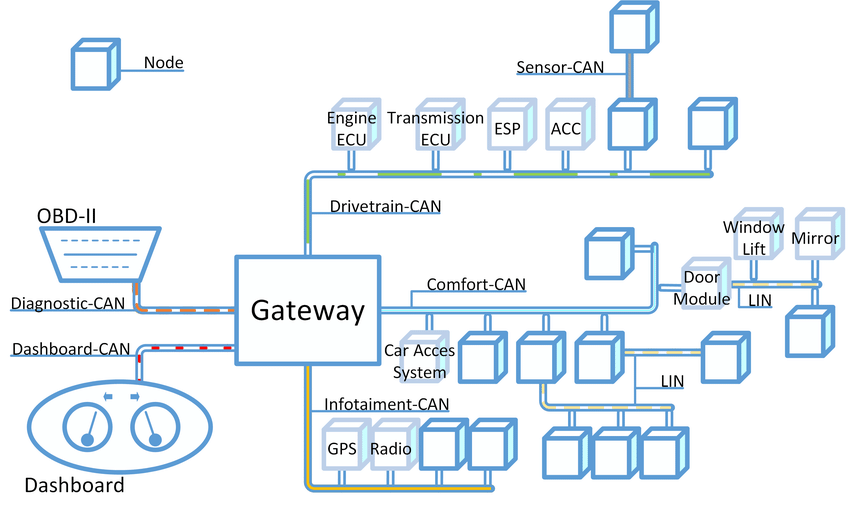
\includegraphics[width=\linewidth]{src/VehicleNetwork.png}
    \caption{Ejemplo de red vehicular con múltiples buses CAN interconectados mediante un gateway}
    \label{fig:vehicle_network}
\end{figure}
\newpage
\section{Implementación Práctica en STM32}\label{sec:implementation}
Los microcontroladores STM32 integran de forma nativa un periférico controlador CAN: \textbf{bxCAN} (\textit{Basic Extended CAN}) en familias como F1, F4 y F103, o el más moderno \textbf{FDCAN} en familias G4, H7 y L5, este último con soporte completo para CAN FD. En ambos casos, es necesario un transceptor externo (por ejemplo, TJA1050 o SN65HVD230) entre los pines TX/RX del periférico y el bus físico CAN\_H/CAN\_L.

\textbf{¿Qué hace el transceptor?}
El controlador CAN del STM32 trabaja con señales digitales de 3.3 V (TX y RX). El transceptor se encarga de:
\begin{itemize}
    \item Convertir esas señales al nivel diferencial de CAN\_H y CAN\_L.
    \item Proteger el microcontrolador frente a perturbaciones del bus.
    \item Adaptar los niveles eléctricos según el estándar ISO 11898.
\end{itemize}

Sin él, no puedes conectar directamente el STM32 al bus CAN.
\subsection{Conexión de Hardware}
La conexión típica involucra los pines \texttt{CAN\_TX} y \texttt{CAN\_RX} del microcontrolador hacia el transceptor, y las salidas diferenciales del transceptor hacia el bus con su resistencia de terminación de \SI{120}{\ohm} en cada extremo físico del bus (no en cada nodo).
\begin{comment}
    
%--------------------------------------------------------------%
 IMAGEN 7: Buscar un diagrama esquemático de conexión entre un  
 microcontrolador STM32 (pines CAN_TX, CAN_RX), un transceptor  
 CAN (p. ej. TJA1050 o SN65HVD230) y el bus físico CAN_H/CAN_L, 
 incluyendo las resistencias de terminación de 120 ohms en cada 
 extremo del bus.                                                
 Buscar en: "STM32 CAN transceiver TJA1050 schematic 120 ohm     
 termination", SN65HVD230 CAN bus wiring diagram STM32           
%--------------------------------------------------------------%
\end{comment}

\begin{figure}[!h]
    \centering
    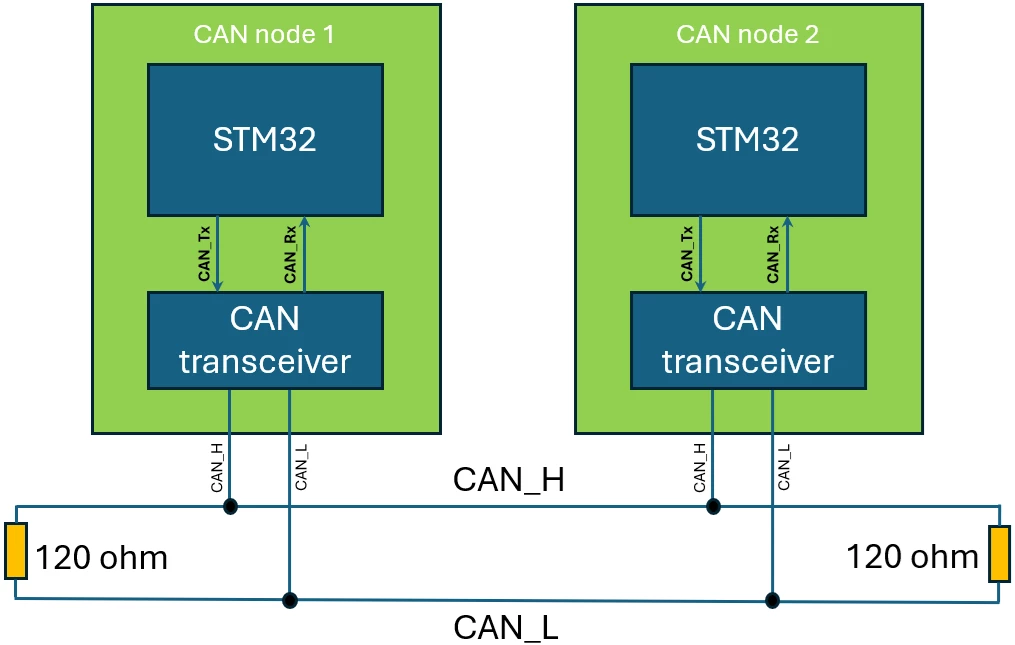
\includegraphics[width=\linewidth]{src/STM32Schematic.png}
    \caption{Esquemático de conexión STM32 + transceptor CAN + bus terminado}
    \label{fig:stm32_schematic}
\end{figure}

Es recomendable utilizar el modulo \textbf{SN65HVD230} debido a que trabaja a 3.3 V, es compatible con el nivel lógico del STM32 y soporta velocidades de hasta 1 Mbit/s. Además, su consumo es bajo y tiene protección contra cortocircuitos y sobrevoltajes.
\subsection{Configuración e Inicialización (bxCAN)}
El siguiente ejemplo ilustra, a nivel conceptual, la configuración mínima del periférico bxCAN utilizando HAL para transmitir una trama estándar con identificador y dos bytes de datos.
\newpage


\codeheader{main.c -- Inicialización y envío bxCAN}
\begin{lstlisting}[style=algorithmstyle]
CAN_HandleTypeDef hcan1;
CAN_TxHeaderTypeDef TxHeader;
uint8_t TxData[8];
uint32_t TxMailbox;

void CAN1_Config(void) {
    hcan1.Instance = CAN1;
    hcan1.Init.Prescaler = 4;              // Ajustar segun APB1 clock
    hcan1.Init.Mode = CAN_MODE_NORMAL;
    hcan1.Init.SyncJumpWidth = CAN_SJW_1TQ;
    hcan1.Init.TimeSeg1 = CAN_BS1_13TQ;
    hcan1.Init.TimeSeg2 = CAN_BS2_2TQ;      // Bit rate objetivo: 500 kbit/s
    hcan1.Init.TimeTriggeredMode = DISABLE;
    hcan1.Init.AutoBusOff = DISABLE;
    hcan1.Init.AutoWakeUp = DISABLE;
    hcan1.Init.AutoRetransmission = ENABLE;
    hcan1.Init.ReceiveFifoLocked = DISABLE;
    hcan1.Init.TransmitFifoPriority = DISABLE;

    HAL_CAN_Init(&hcan1);

    // Filtro: aceptar todos los identificadores (ejemplo simple)
    CAN_FilterTypeDef sFilterConfig;
    sFilterConfig.FilterBank = 0;
    sFilterConfig.FilterMode = CAN_FILTERMODE_IDMASK;
    sFilterConfig.FilterScale = CAN_FILTERSCALE_32BIT;
    sFilterConfig.FilterIdHigh = 0x0000;
    sFilterConfig.FilterIdLow = 0x0000;
    sFilterConfig.FilterMaskIdHigh = 0x0000;
    sFilterConfig.FilterMaskIdLow = 0x0000;
    sFilterConfig.FilterFIFOAssignment = CAN_FILTER_FIFO0;
    sFilterConfig.FilterActivation = ENABLE;
    HAL_CAN_ConfigFilter(&hcan1, &sFilterConfig);

    HAL_CAN_Start(&hcan1);
}

void CAN1_SendFrame(uint16_t id, uint8_t byte0, uint8_t byte1) {
    TxHeader.StdId = id;         // Identificador de 11 bits: define la prioridad
    TxHeader.ExtId = 0;
    TxHeader.IDE = CAN_ID_STD;   // Formato estandar
    TxHeader.RTR = CAN_RTR_DATA; // Trama de datos (no remota)
    TxHeader.DLC = 2;            // 2 bytes de payload
    TxHeader.TransmitGlobalTime = DISABLE;

    TxData[0] = byte0;
    TxData[1] = byte1;

    HAL_CAN_AddTxMessage(&hcan1, &TxHeader, TxData, &TxMailbox);
}
\end{lstlisting}

Puntos clave del ejemplo:
\begin{itemize}
    \item El \texttt{Prescaler}, \texttt{TimeSeg1} y \texttt{TimeSeg2} determinan la velocidad de bit (\textit{bit rate}) resultante a partir del reloj APB1; deben calcularse de modo que todos los nodos de la red compartan exactamente la misma velocidad nominal.
    \item El campo \texttt{StdId} corresponde directamente al identificador de arbitraje descrito en la sección \ref{sec:frame}: entre menor su valor, mayor prioridad tendrá la trama en el bus.
    \item \texttt{AutoRetransmission = ENABLE} delega al hardware bxCAN el reintento automático de una trama tras perder el arbitraje o detectar un error, replicando el comportamiento estándar del protocolo.
\end{itemize}

\subsection{Recepción por Interrupción}
Para recibir mensajes es recomendable habilitar la interrupción de FIFO 0 con nuevo mensaje pendiente (\texttt{CAN\_IT\_RX\_\allowbreak FIFO0\_MSG\_\allowbreak PENDING}) y sobrescribir el callback \texttt{HAL\_CAN\_RxFifo0\allowbreak MsgPendingCallback}, leyendo la trama con \texttt{HAL\_CAN\_\allowbreak GetRxMessage} para evitar sondeo (\textit{polling}) continuo del periférico y reducir el uso de CPU, de forma análoga a las mejoras de DMA/interrupciones discutidas para otros periféricos SPI.

\section{Referencias y Recursos para Profundizar}\label{sec:references}
A continuación se listan fuentes primarias y recursos prácticos para profundizar en lo revisado en este reporte, organizados por categoría.

\subsection{Estándares y especificaciones oficiales}
\begin{itemize}
    \item Bosch, \textit{CAN Specification Version 2.0} (documento original, formatos estándar y extendido): \url{http://esd.cs.ucr.edu/webres/can20.pdf}
    \item CAN in Automation (CiA), \textit{History of CAN Technology} (resumen histórico y estado actual de ISO 11898/CAN FD/CAN XL): \url{https://www.can-cia.org/can-knowledge/history-of-can-technology}
    \item CAN in Automation (CiA), portal oficial de la organización (CANopen, perfiles de dispositivo, documentación): \url{https://www.can-cia.org/}
    \item Wikipedia, \textit{CAN bus} (panorama general con referencias cruzadas a CAN FD y CAN XL): \url{https://en.wikipedia.org/wiki/CAN_bus}
\end{itemize}

\subsection{Datasheets de transceptores (capa física)}
\begin{itemize}
    \item NXP, \textit{TJA1050 -- High Speed CAN Transceiver}: \url{https://www.nxp.com/docs/en/data-sheet/TJA1050.pdf}
    \item Texas Instruments, \textit{SN65HVD230/231/232 -- 3.3V CAN Bus Transceivers}: \url{https://www.ti.com/lit/ds/symlink/sn65hvd230.pdf}
\end{itemize}

\subsection{Implementación en STM32 (bxCAN/HAL)}
\begin{itemize}
    \item ST Community, \textit{Using CAN (bxCAN) in Normal mode with STM32 microcontrollers -- Part 1} (teoría, hardware y configuración): \url{https://community.st.com/t5/stm32-mcus/using-can-bxcan-in-normal-mode-with-stm32-microcontrollers-part/ta-p/800502}
    \item ST Community, \textit{Using CAN (bxCAN) in Normal mode with STM32 microcontrollers -- Part 2} (ejemplo práctico completo): \url{https://community.st.com/t5/stm32-mcus/using-can-bxcan-in-normal-mode-with-stm32-microcontrollers-part/ta-p/810853}
    \item ST Community, \textit{CAN (bxCAN) bit time configuration on STM32 MCUs} (cálculo de \texttt{CAN\_BTR}, prescaler y segmentos de tiempo): \url{https://community.st.com/t5/stm32-mcus/can-bxcan-bit-time-configuration-on-stm32-mcus/ta-p/689864}
    \item ST Community, \textit{Guide to CAN (bxCAN/CAN2.0) configuration in Loop back mode on STM32 MCUs} (útil para probar sin un segundo nodo físico): \url{https://community.st.com/stm32-mcus-60/guide-to-can-bxcan-can2-0-configuration-in-loop-back-mode-on-stm32-mcus-146788}
    \item ControllersTech, \textit{STM32 CAN Bus Communication in Normal Mode: CubeMX Setup \& HAL Code} (tutorial con proyecto descargable, dos nodos STM32 + MCP2551): \url{https://controllerstech.com/can-protocol-in-stm32/}
\end{itemize}

\subsection{Herramientas y librerías de software}
\begin{itemize}
    \item \textit{python-can}, librería de Python para CAN sobre SocketCAN, PCAN, Vector, Kvaser, etc.: \url{https://python-can.readthedocs.io/}
    \item \textit{python-can}, repositorio en GitHub: \url{https://github.com/hardbyte/python-can}
    \item Documentación de la interfaz SocketCAN dentro de python-can (creación de interfaces virtuales \texttt{vcan}, uso de \texttt{cansend}/\texttt{candump}): \url{https://python-can.readthedocs.io/en/stable/interfaces/socketcan.html}
\end{itemize}

\begin{comment}
    Resources
    https://honda-tech.com/forums/tech-misc-15/any-information-honda-can-bus-2825633/
    https://github.com/marcellatwin/honda-canbus-project
    https://www.cjindustriesaustralia.com/blogs/canbus-settings/honda-canbus-settings-cr-v-fit-jazz-civic-odyssey-accord-city-etc?srsltid=AfmBOooJQAEVHB_3T1qvhvghN4wXMAKU_n9l7jSUo22kCEmljVZEn51B
    https://forum.autosportlabs.com/viewtopic.php?t=6148
    https://arxiv.org/html/2408.09265v1
    https://github.com/commaai/opendbc/blob/master/README.md#how-to-port-a-car
\end{comment}
\section{Conclusión}\label{sec:conclusion}
El protocolo CAN se ha consolidado durante casi cuatro décadas como el bus de comunicación de referencia en sistemas embebidos distribuidos, gracias a un diseño elegante que resuelve de forma determinista el acceso múltiple al medio mediante arbitraje bit a bit, y a un sistema de detección de errores excepcionalmente robusto para el bajo costo de su capa física. Si bien su ancho de banda y tamaño de carga útil resultan limitados frente a las demandas actuales de los vehículos autónomos y conectados, su evolución hacia CAN FD -y en desarrollo, CAN XL- demuestra la vigencia del enfoque original. Para el trabajo práctico con microcontroladores STM32, el periférico bxCAN/FDCAN ofrece una vía directa y bien soportada por HAL para integrar nodos CAN en proyectos de instrumentación, robótica o redes de sensores distribuidos.

\end{document}